% Template for NIME 2023

% Modified by Adnan Marquez-Borbon 30 November 2022
% Modified by Courtney Reed 28 November 2022
% Modified by Joe Wright 14 December 2019
% Modified by Niccolò Granieri 10 October 2018 
% Modified by Angelo Fraietta 23 December 2018
% Modified by Angelo Fraietta 22 November 2018
% Modified by Rodrigo Schramm on 22 September 2018
% Modified by Luke Dahl on 17 October 2-17
% Modified by Cumhur Erkut on <2016-10-11 Tue>
% Modified by Edgar Berdahl on 5 November 2014
% Modified by Baptiste Caramiaux on 25 November 2013
% Modified by Kyogu Lee on 7 October 2012
% Modified by Georg Essl on 7 November 2011
%
% Based on "sig-alternate.tex" V1.9 April 2009
% This file should be compiled with "nime-alternate.cls"

\documentclass{nime-alternate} % Uncomment when publishing final version
\usepackage{parskip}
% Uncomment only one of the ones below
\usepackage{anonymize} 		   %Uncomment this line to publish
% \usepackage[blind]{anonymize}%Uncomment this line for blind review

% Package that enables the use of accents and non 
% standard characters
\usepackage[utf8]{inputenc}

\begin{document}

% --- Author Metadata here ---
%\conferenceinfo{NIME'17,}{May 15-19, 2017, Aalborg University Copenhagen, Denmark.}
%\conferenceinfo{NIME'18,}{June 3-6, 2018, Blacksburg, Virginia, USA.}
%\conferenceinfo{NIME'19,}{June 3-6, 2019, Federal University of Rio Grande do Sul, ~~~~~~  Porto Alegre,  Brazil.}
% \conferenceinfo{NIME'20,}{July 21-25, 2020, Royal Birmingham Conservatoire, ~~~~~~~~~~~~ Birmingham City University, Birmingham, United Kingdom.}
%\conferenceinfo{NIME'22,}{June 28 - July 1, 2022, Waipapa Taumata Rau, T\={a}maki ~~~~~~~~ Makaurau, Aotearoa}

\conferenceinfo{NIME'24,}{4--6 September, Utrecht, The Netherlands.}

\title{Text-to-Playable-Sound: Digital Instrument based on Latent Diffusion}

% You need the command \numberofauthors to handle the 'placement
% and alignment' of the authors beneath the title.
%
% For aesthetic reasons, we recommend 'three authors at a time'
% i.e. three 'name/affiliation blocks' be placed beneath the title.
%
% NOTE: You are NOT restricted in how many 'rows' of
% "name/affiliations" may appear. We just ask that you restrict
% the number of 'columns' to three.
%
% Because of the available 'opening page real-estate'
\label{key}% we ask you to refrain from putting more than six authors
% (two rows with three columns) beneath the article title.
% More than six makes the first-page appear very cluttered indeed.
%
% Use the \alignauthor commands to handle the names
% and affiliations for an 'aesthetic maximum' of six authors.
% Add names, affiliations, addresses for
% the seventh etc. author(s) as the argument for the
% \additionalauthors command.
% These 'additional authors' will be output/set for you
% without further effort on your part as the last section in
% the body of your article BEFORE References or any Appendices.

\numberofauthors{8} %  in this sample file, there are a *total*
% of EIGHT authors. SIX appear on the 'first-page' (for formatting
% reasons) and the remaining two appear in the \additionalauthors section.
%
\author{
% You can go ahead and credit any number of authors here,
% e.g. one 'row of three' or two rows (consisting of one row of three
% and a second row of one, two or three).
%
% The command \alignauthor (no curly braces needed) should
% precede each author name, affiliation/snail-mail address and
% e-mail address. Additionally, tag each line of
% affiliation/address with \affaddr, and tag the
% e-mail address with \email.
%
% 1st. author
\alignauthor
\anonymize{Pierre-Louis Suckrow}\\
        \affaddr{\anonymize{Universität der Künste Berlin}}\\
        \affaddr{\anonymize{M.A. Design \& Computation}}\\
        \affaddr{\anonymize{c/o Präsident der UdK}}\\
        \affaddr{\anonymize{Einsteinufer 43}}\\
        \affaddr{\anonymize{10587 Berlin, Germany}}\\
       \email{\anonymize{suckrowpierre@gmail.com}}\\
% 2nd. author
\alignauthor
\anonymize{Chris}\\
       \affaddr{\anonymize{LMU Munich}}\\
       \affaddr{\anonymize{P.O. Box 1212}}\\
       \affaddr{\anonymize{Dublin, Ohio 43017-6221}}\\
       \email{\anonymize{webmaster@marysville-ohio.com}}
% 3rd. author
\alignauthor \anonymize{Sylvia}\\
       \affaddr{\anonymize{The Th{\o}rv{\"a}ld Group}}\\
       \affaddr{\anonymize{1 Th{\o}rv{\"a}ld Circle}}\\
       \affaddr{\anonymize{Hekla, Iceland}}\\
       \email{l\anonymize{arst@affiliation.org}}
%\and  % use '\and' if you need 'another row' of author names
% 4th. author
%\alignauthor \anonymize{Lawrence P. Leipuner}\\
%       \affaddr{\anonymize{Brookhaven Laboratories}}\\
%       \affaddr{\anonymize{Brookhaven National Lab}}\\
%       \affaddr{\anonymize{P.O. Box 5000}}\\
%       \email{\anonymize{lleipuner@researchlabs.org}}
% 5th. author
%\alignauthor \anonymize{Sean Fogarty}\\
%       \affaddr{\anonymize{NASA Ames Research Center}}\\
%       \affaddr{\anonymize{Moffett Field}}\\
%       \affaddr{\anonymize{California 94035}}\\
%       \email{\anonymize{fogartys@amesres.org}}
% 6th. author
%\alignauthor \anonymize{Anon Nymous}\\
%       \affaddr{\anonymize{Redacted }}\\
%       \affaddr{\anonymize{8600 Datapoint Drive}}\\
%       \affaddr{\anonymize{San Antonio, Texas 78229}}\\
%       \email{\anonymize{cpalmer@prl.com}}
}
% There's nothing stopping you putting the seventh, eighth, etc.
% author on the opening page (as the 'third row') but we ask,
% for aesthetic reasons that you place these 'additional authors'
% in the \additional authors block, viz.
\additionalauthors{Additional authors: \anonymize{John Smith (The Th{\o}rv{\"a}ld Group,}
email: {\texttt{\anonymize{jsmith@affiliation.org}}}) and \anonymize{Julius P.~Kumquat 
(K. Consortium,} email: {\texttt{\anonymize{jpkumquat@consortium.net}}}).}
\date{30 July 1999}
% Just remember to make sure that the TOTAL number of authors
% is the number that will appear on the first page PLUS the
% number that will appear in the \additionalauthors section.

% For your initial submission you MUST ANONYMIZE the authors.

\maketitle

\begin{abstract}
In this paper we propose a tool for the integration and application of generative artificial intelligence in the field of music production. With the help of selected diffusion models, users can define sounds by textual descriptions, play them back and manipulate them with standardized music production tools. The diffusion models used were evaluated for their suitability in the given context and modified for integration into a digital instrument. Currently available text-to-audio models offer the possibilities for experimental applications. The implementation of a prototype of the digital instrument enables such experiments and the exploration of innovative sound synthesis methods. The resulting user interface allows the user to edit model- and instrument-specific parameters.
\end{abstract} 
\keywords{NIME, proceedings, \LaTeX, template}

% ------- CCS Concepts
% Here is where you enter the CCS Concepts for your paper.
%
% It is strongly recommended that authors view the submission form
% prior to starting to write the paper, which includes information 
% on the CCS Concepts. 
% 
% The 2012 ACM Computing Classification System (CCS) replaces the
% traditional 1998 version, which has served as the de facto 
% standard classification system for the computing field. It is
% being integrated into the search capabilities and visual topic 
% displays of the ACM Digital Library. Please enter the CCS XML code 
% for the classification terms that describe your paper. To get the 
% XML code, please use the following procedure, which is
% demonstrated using three NIME-related example terms: Applied
% computing~Sound and music computing, Applied computing~Performing
% arts, and Information systems~Music retrieval.
%
% 1) Browse to the website http://dl.acm.org/ccs_flat.cfm.
% 2) Select one to three classification terms from the website that
%    describe your paper (e.g. for the example paper Applied
%    computing~Sound and music computing, Applied 
%    computing~Performing arts, and Information systems~Music
%    retrieval.).
% 3) For each classification you need to select the relevance
%    (e.g. for this example, Sound and music computing is "high",
%    Performing arts is "low", and Music retrieval is "Medium")
% 4) Once you have selected the last term, click on "view CCS Tex
%    Code". This will generate some code, which includes some CCSXML
%    and some lines beginning with \ccsdesc.
% 5) Keep all of this code, as you will need it for entering into
%    the Precision Conference System paper submission form.
% 6) For this document, keep only the \ccsdesc lines. Here is what
%    you would paste for the classification example:

\ccsdesc[500]{Applied computing~Sound and music computing}
\ccsdesc[100]{Applied computing~Performing arts}
\ccsdesc[300]{Information systems~Music retrieval}

% this line creates the CCS Concepts section.
\printccsdesc

\textbf{Please read the comments starting on line 140 of the nime-template.tex file to see how to create the CCS Concept Classifications!} % Remove this line in your paper!

\section{Introduction (Chris)}
Sound libraries offer artists the opportunity to quickly access a large number of stored sounds. However, these libraries can also have limitations as artists are reliant on the work of other producers. The ability to instantly create any
sound with just a textual description not only offers artists the benefits of time and labor savings. It also allows them to create unique and customized sounds for every situation.

Research question(s) / Problem

\section{Related Work (Pierre)}
The development of an instrument that enables sound synthesis through artificial intelligence was pursued in 2023 as part of the ”Neural Audio Plugin” competition organised by Juce [?] organised the ”Neural Audio Plugin” competi-
tion. In particular, the project VroomAi [?] was charac-
terised by the use of the same C++ audio framework as
in this project. In VroomAi, a digital instrument was de-
veloped that enables the input of a user-specific prompt for
sound generation via a user interface. This sound can then
be made playable by using a Sampler.
VroomAi provides two models: The model AudioLDM
[?], which is also used in this work, and the model AudioLM
[?]. The model AudioLDM2 had not yet been published by
the publication date of this paper and is therefore not used.
The architecture implemented in VroomAi is similar to the
implementation presented in this paper. Its main purpose
is to execute the models and generate sounds. For this
purpose, a Gradio server [?] is used, which executes the
model locally.

- Latent Diffusion 
(- Überleitung was macht einen Klang aus (gegenüber Rauschen))
- AudioLDM
- VroomAI - was unterscheidet uns davon?

\section{Design}
To ensure the developed instrument exhibits minimal latency during use, the predominant choice for programming language in real-time audio applications C++ \cite{doumler_c_2015, boulanger_audio_2011} is being used in conjunction with the \emph{JUCE}\footnote{\url{https://juce.com/}} framework. Enriching the framework with the Module \emph{PluginGuiMagic}\footnote{\url{https://foleysfinest.com/developer/pluginguimagic/}} helped in the development of the GUI. 
\newline

\emph{JUCE} is an open-source C++ codebase, enabling the creation of standalone software across multiple platforms and different plugin formats. The framework provides an abstraction layer for audio processing and \emph{MIDI} from native audio devices on each platform or a Host-DAW. The digital signal processing (DSP) library offered by \emph{JUCE} facilitates rapid prototyping and implementation of various audio effects, filters, instruments, and generators. Additionally, \emph{JUCE} offers a multitude of classes addressing common challenges in audio project development, including the management of graphics, sound, user interaction, and network communication. \cite{juce, robinson_getting_2013}
\newline


In order to utilize the diffusion models \emph{AudioLDM} and \emph{AudioLDM2} within the digital instrument framework of \emph{JUCE}, one must enable the inference of these models from the instrument's C++ source code. The in \cite{oli_larkin_machine_2023} discussed favorable generation of binary representations for the models in formats such as ONNX \footnote{\url{https://onnx.ai/}} or Torchscript \footnote{\url{https://pytorch.org/docs/stable/jit.html}} was not feasible, due to their complex structure and reliance of different sub-models. Consequently, we opted to operate the models on a locally hosted FastAPI\footnote{\url{https://fastapi.tiangolo.com/}} server. This server hosts instances of the on HuggingFace shared \emph{AudioLDM}\footnote{\url{https://huggingface.co/docs/diffusers/main/en/api/pipelines/audioldm}} models "audioldm-s-full-v2", "audioldm-m-full", "audioldm-l-full", and the \emph{AudioLDM2}\footnote{\url{https://huggingface.co/docs/diffusers/main/en/api/pipelines/audioldm2}} models "audioldm2", "audioldm2-large", "audioldm2-music". These models can be initialized through an API endpoint, by also specifying a system-specific \emph{torch device}. For silicone architectures, "mps" is the recommended torch device, whereas "cuda" is suitable for Nvidia\footnote{\url{https://www.nvidia.com/}} GPUs, when supported, and "cpu" for other architectures. Upon initialization, the model can be infered through a dedicated API endpoint by defining a prompt, a negative prompt, the desired audio length, the number of inference steps, the guidance scale, and an optional 8-Byte large seed. The endpoint then generates the audio signal based on these parameters and returns it as a \emph{Base64} encoded audio. This encoded signal can subsequently be processed in the C++ source code of the digital instrument. All the mentioned parameters, models, torch-devices and the port for the api can be set via the provided GUI (\ref{})
\newline

Once generated the audio signal is being displayed by showing its waveform and spectogramm and loaded into a sampler, which was implemented by augmenting the provided by \emph{Juce} class for a basic sampler with the ability to pitch shift the sample continously up and down an octave and also utilize the pitch bender of a keyboard with the standard range of two semitones. While the sound is being played the GUI gives the possibility to alter the envelope of the sound by seting the Attack, Decay, Sustain and Release. Additionaly the gain can be set and the instrument tuned so that the pitch of the generated signal matches the MIDI mapping. 

\begin{figure}[h]
  \centering
  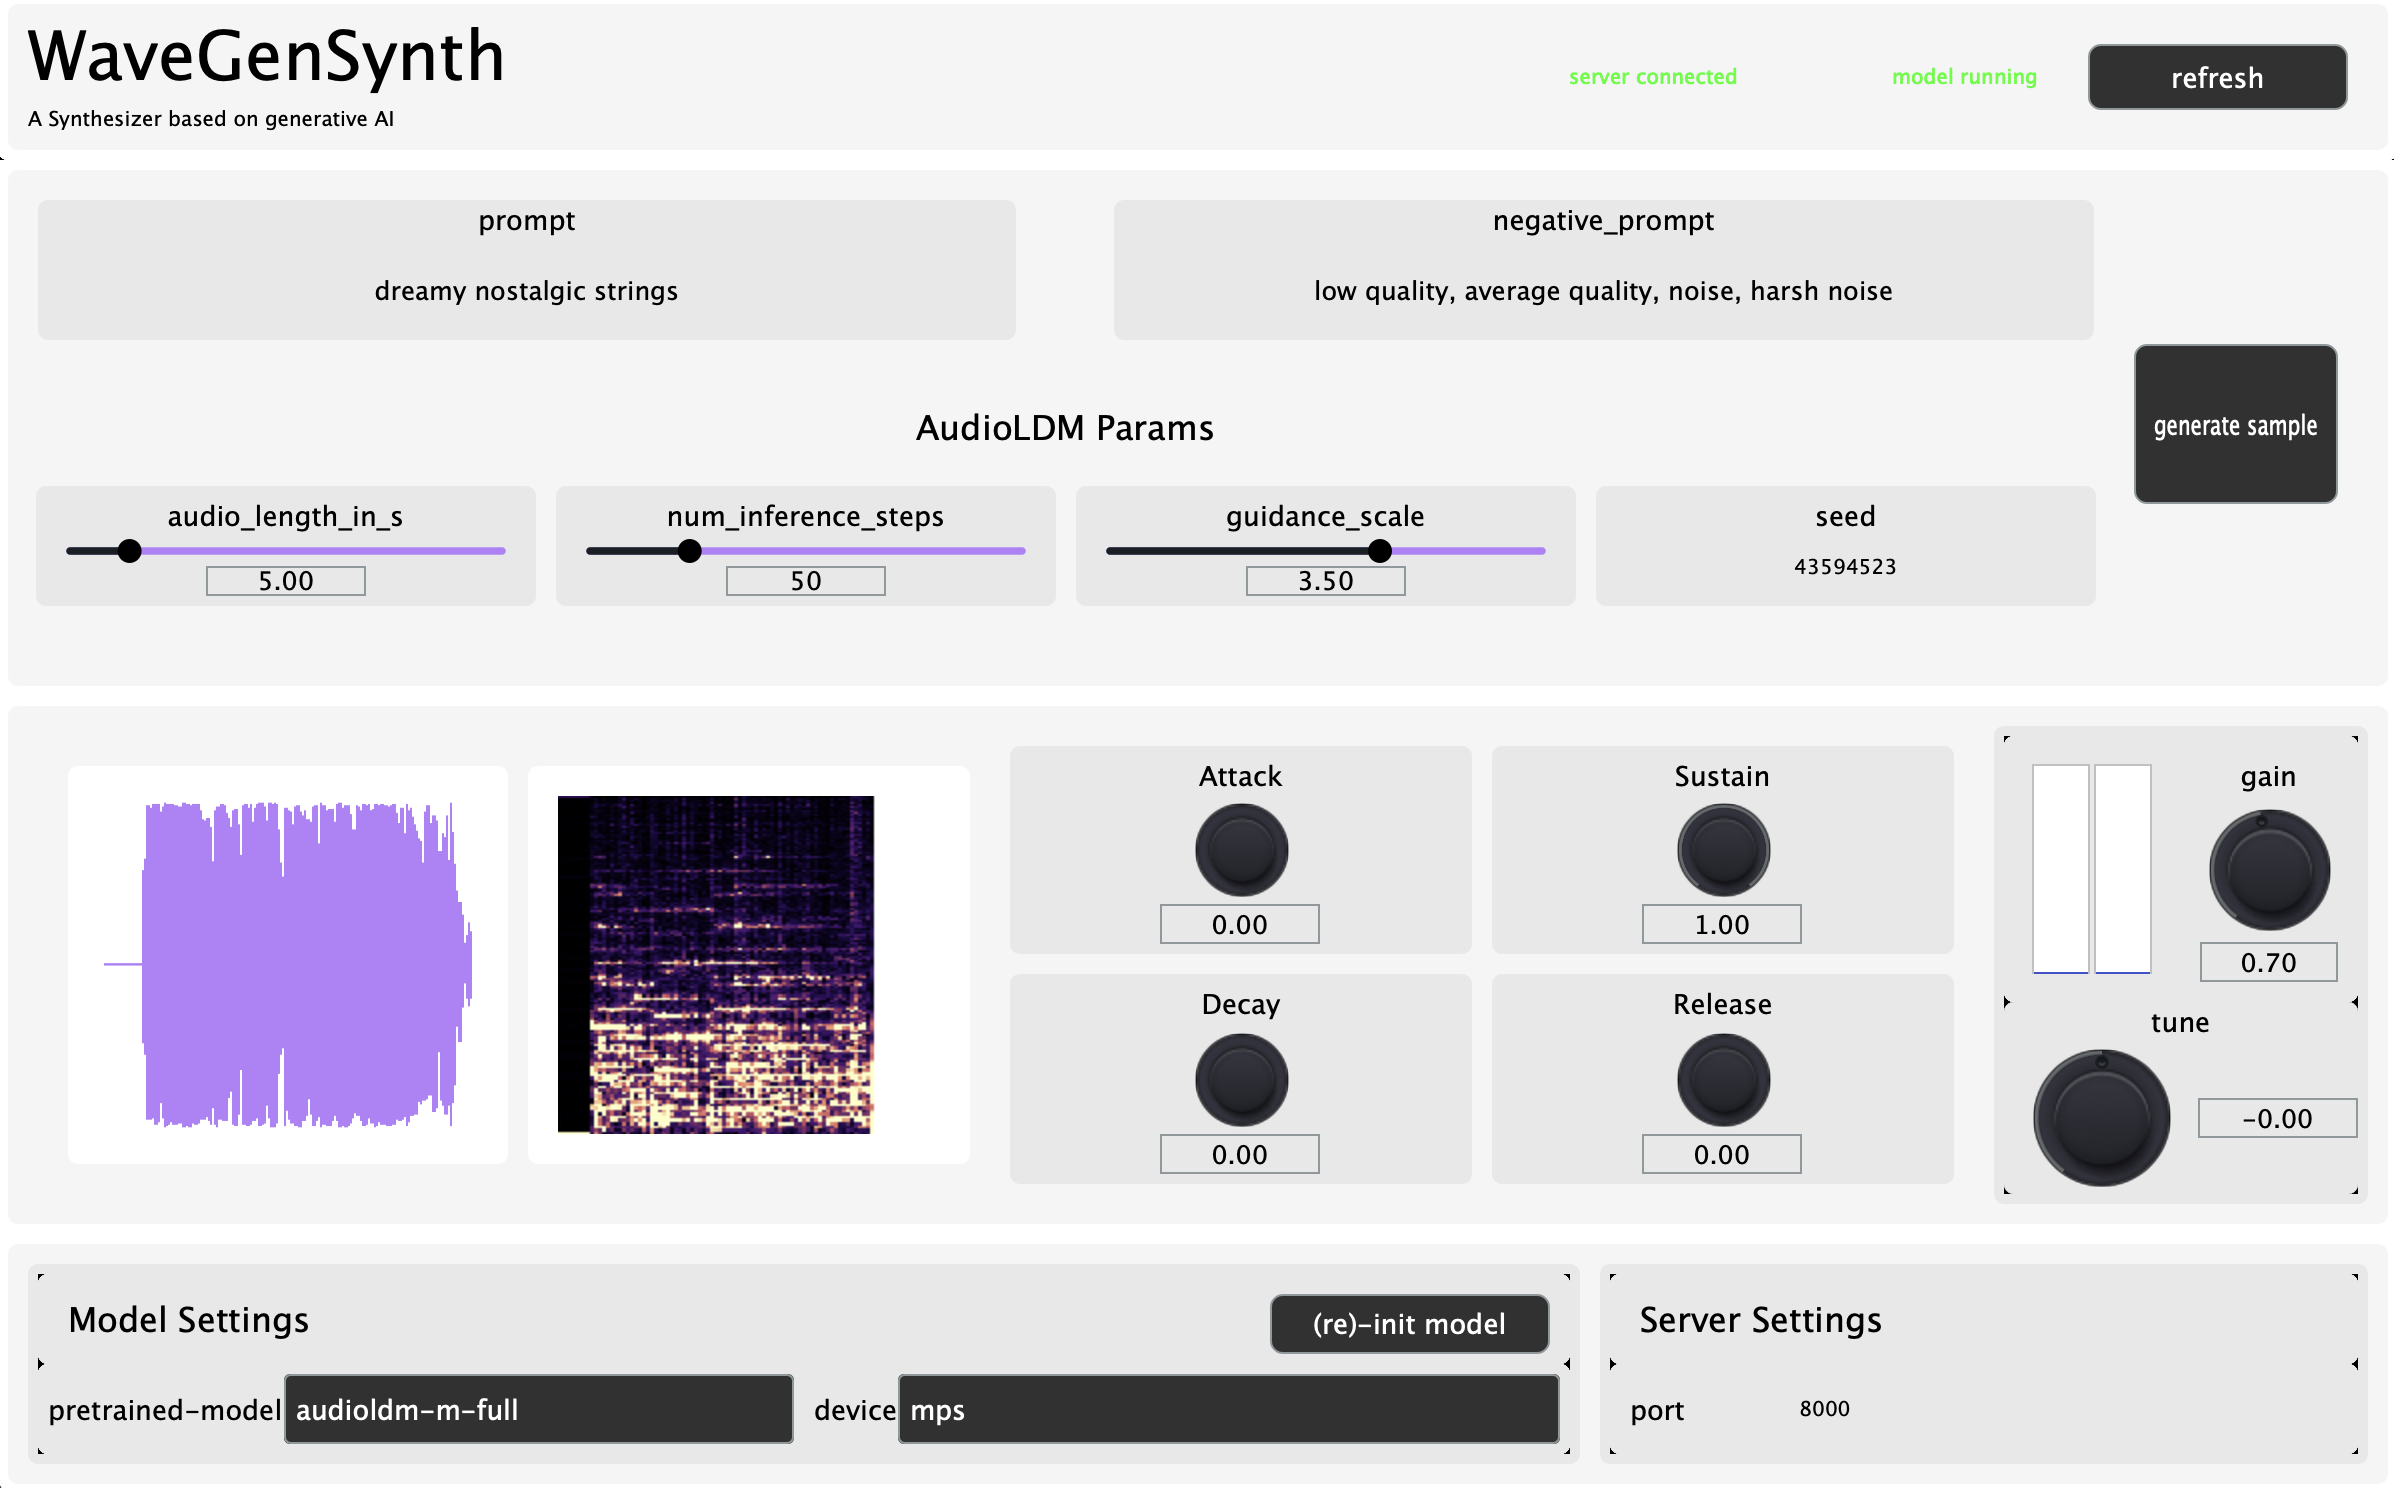
\includegraphics[width=.5\textwidth]{graphics/synth.png}
  \caption[GUI]{GUI}
  \label{fig:synth}
\end{figure} 

For macOS\footnote{\url{https://www.apple.com/de/macos/}}, a \emph{.app} application file, a \emph{VST3}, and an \emph{AU} file could be generated. To simplify the installation of these files for users, they were bundled into a \emph{pkg} installation file.

The FastAPI server was compiled into an application using pyinstaller\footnote{\url{https://pyinstaller.org/en/stable/}}, allowing users to open it effortlessly by integrating all necessary dependencies into one package \cite{pyinstaller}. However, as all required modules are included, for example, the Silicon server originally a $5$ KB script results in a file size of $450$ MB. The increase in storage requirement is substantial but indispensable for distributing and publishing the server and thus a usable instrument. If the generated server applications exhibit unstable performance or problems on a system, the server script can also be executed in a specified Conda\footnote{\url{https://www.anaconda.com/}} environment.

The digital instrument was tested both on macOS with Silicon and Intel chipset. When using the server application on Intel Macs with a mandatory torch-device "cpu", poor and unstable performance was observed. In this case, it is advisable to run the script for the server in the Conda environment with the specified Python modules.

\section{Evaluation of AudioLDM Models}
Short evaluation of the various models
(Pierre macht Auswertung nochmal und Chris macht stat. Auswertung)

\section{Discussion (Pierre und Chris)}
Whilst we have found that AudioLDM2 works well with longer audio sequences, short samples are not the main focus of AudioLDM and consequently the short samples produced lack quality.


\section{Conclusions (Pierre und Chris)}
This paragraph will end the body of this sample document.
Remember that you might still have Acknowledgments or
Appendices; brief samples of these
follow.  There is still the Bibliography to deal with; and
we will make a disclaimer about that here: with the exception
of the reference to the \LaTeX\ book, the citations in
this paper are to articles which have nothing to
do with the present subject and are used as
examples only.
%\end{document}  % This is where a 'short' article might terminate

%ACKNOWLEDGMENTS are optional
\section{Acknowledgments (Pierre)}
This section is optional; it is a location for you
to acknowledge grants, funding, editing assistance and
what have you.  In the present case, for example, the
authors would like to thank Gerald Murray of ACM for
his help in codifying this \textit{Author's Guide}
and the \textbf{.cls} and \textbf{.tex} files that it describes.

JUCE
Plugin GUI Magic - Daniel
AudioLDM



\section{Ethical Standards (Chris)}
To ensure objectivity and transparency in research and to ensure that accepted principles of ethical and professional conduct have been followed, authors should include a section “Ethical Standards” before the References, including (if relevant): information regarding sources of funding, potential conflicts of interest (financial or non-financial), informed consent if the research involved human participants, statement on welfare of animals if the research involved animals.





%
% The following two commands are all you need in the
% initial runs of your .tex file to
% produce the bibliography for the citations in your paper.
\bibliographystyle{abbrv}

	\bibliography{nime-references} 


% You must have a proper ".bib" file
%  and remember to run:
% latex bibtex latex latex
% to resolve all references
%
% ACM needs 'a single self-contained file'!
%
%APPENDICES are optional
\appendix
%Appendix A
\section{Headings in Appendices}
The rules about hierarchical headings discussed above for
the body of the article are different in the appendices.
In the \textbf{appendix} environment, the command
\textbf{section} is used to
indicate the start of each Appendix, with alphabetic order
designation (i.e. the first is A, the second B, etc.) and
a title (if you include one).  So, if you need
hierarchical structure
\textit{within} an Appendix, start with \textbf{subsection} as the
highest level. Here is an outline of the body of this
document in Appendix-appropriate form:
\subsection{Introduction}
\subsection{The Body of the Paper}
\subsubsection{Type Changes and  Special Characters}
\subsubsection{Math Equations}
\paragraph{Inline (In-text) Equations}
\paragraph{Display Equations}
\subsubsection{Citations}
\subsubsection{Tables}
\subsubsection{Figures}
\subsubsection{Theorem-like Constructs}
\subsubsection*{A Caveat for the \TeX\ Expert}
\subsection{Conclusions}
\subsection{Acknowledgments}
\subsection{Additional Authors}
This section is inserted by \LaTeX; you do not insert it.
You just add the names and information in the
\texttt{{\char'134}additionalauthors} command at the start
of the document.
\subsection{References}
Generated by bibtex from your ~.bib file.  Run latex,
then bibtex, then latex twice (to resolve references)
to create the ~.bbl file.  Insert that ~.bbl file into
the .tex source file and comment out
the command \texttt{{\char'134}thebibliography}.

% This next section command marks the start of
% Appendix B, and does not continue the present hierarchy
\section{More Help for the Hardy}
The sig-alternate.cls file itself is chock-full of succinct
and helpful comments.  If you consider yourself a moderately
experienced to expert user of \LaTeX, you may find reading
it useful but please remember not to change it.

%%% Place this command where you want to balance the columns on the last page. 
%\balancecolumns 

% That's all folks!
\end{document}
